
\documentclass{beamer}
\beamertemplatenavigationsymbolsempty
\graphicspath{ {./images/} }
\setbeamercolor{section number projected}{bg=red,fg=white}
\setbeamercolor{subsection number projected}{bg=red}
\setbeamertemplate{itemize items}[triangle]
\setbeamercolor{itemize item}{fg=red}
\setbeamertemplate{itemize subitem}[circle]
\setbeamercolor{itemize subitem}{fg=red}
\usepackage{multicol}

\mode<presentation>
{
  	\usetheme{CambridgeUS}
  	\setbeamercovered{transparent}
}

\usepackage[english]{babel}
\usepackage[utf8]{inputenc}
\usepackage{times}
\usepackage[T1]{fontenc}

\title[Face recognition]
{Multiple face recognition in images}

\author[Simone Caldarella]
{Simone~Caldarella }

\institute[University of Brescia] 
{
  	IEEE Student Branch Brescia\\
  	University of Brescia
}

\date[IEEE Student Branch 2018] 
{
	Presentation on Convolutional Neural Networks, 2018
}

\subject{Theoretical Computer Science}

\AtBeginSubsection[]
{
 	\begin{frame}<beamer>{Outline}
		\begin{multicols}{2}
   			\tableofcontents[currentsection,currentsubsection]
		\end{multicols}
  	\end{frame}
}

\begin{document}

\begin{frame}
 	\titlepage
\end{frame}

\begin{frame}{Outline}
	\begin{multicols}{2}
  		\tableofcontents
	\end{multicols}
\end{frame}

\section{Introduction}

\subsection{Machine learning}

\begin{frame}{What does machine learning means?}
	\begin{itemize}
		\setbeamertemplate{itemize items}[triangle]
		\setbeamercolor{itemize item}{fg=red}
  		\item
    			Is this a \textbf{neural network} or a \textbf{graph}?
	\end{itemize}
	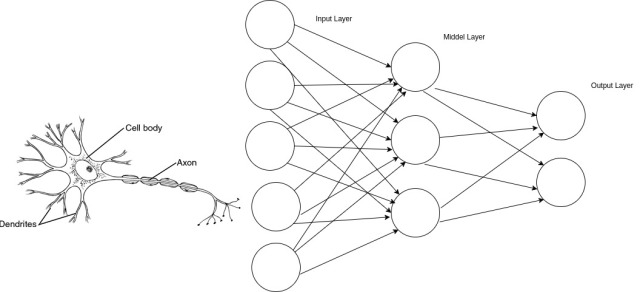
\includegraphics[scale=0.5]{neuralNet}
\end{frame}

\begin{frame}{What does machine learning means?}
	\begin{itemize}
		\setlength\itemsep{1em}
		\setbeamertemplate{itemize item}[triangle]
		\setbeamercolor{itemize item}{fg=red}
  		\item 
			The concept of \texttt{training}
    			\begin{itemize}
				\setbeamertemplate{itemize subitem}[circle]
				\setbeamercolor{itemize subitem}{fg=red}
    				\item
      					Minimize the loss
    				\item    
      					Loss functions
   				\item
					Weights update
			\end{itemize}
		\item
    			The importance of a large and well organized dataset
    			\begin{itemize}
				\setbeamertemplate{itemize subitem}[circle]
				\setbeamercolor{itemize subitem}{fg=red}
   				\item 
					Common problems
    				\item 
					Cognitive bias
    			\end{itemize}
 	 \end{itemize}
\end{frame}

\subsection{Tensorflow and OpenCv}

\begin{frame}{Tensorflow and OpenCv}
	\begin{itemize}
		\setlength\itemsep{1em}
		\setbeamertemplate{itemize item}[triangle]
		\setbeamercolor{itemize item}{fg=red}
		\item 
			Tensorflow and computational graph concept
	\end{itemize}
	\begin{center}
    		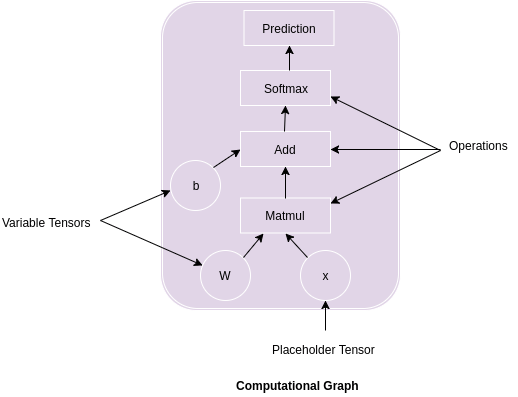
\includegraphics[scale=0.4]{comp}
	\end{center}
\end{frame}

\begin{frame}{Tensorflow and OpenCv}
	\begin{itemize}
		\setlength\itemsep{1em}
		\setbeamertemplate{itemize item}[triangle]
		\setbeamercolor{itemize item}{fg=red}
		\item 
			Low level and high level API
			\begin{itemize}
				\setbeamertemplate{itemize subitem}[circle]
				\setbeamercolor{itemize subitem}{fg=red}
				\item 
					Tensorflow functions
				\item 
					Keras and tflearn
			\end{itemize}
		\item 
			OpenCv "magic" detection algorithm
			\begin{itemize}
				\setbeamertemplate{itemize subitem}[circle]
				\setbeamercolor{itemize subitem}{fg=red}
				\item 
					HaarCascadeClassifier
				\item 
					Dlib library for facial features detection
			\end{itemize}
	\end{itemize}
\end{frame}



\section{Image classification}

\subsection{Convolutional Neural Network}

\begin{frame}{Convolutional Neural Network}
	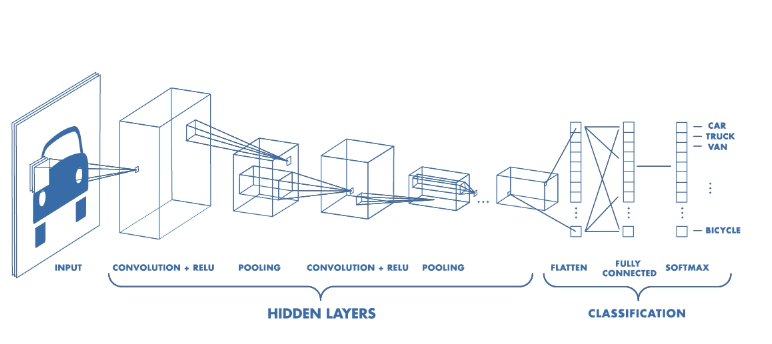
\includegraphics[scale=0.45]{CNN}
\end{frame}

\begin{frame}{Convolutional layers}
	\begin{itemize}
		\setlength\itemsep{1em}
		\setbeamertemplate{itemize item}[triangle]
		\setbeamercolor{itemize item}{fg=red}
		\item 
			Convolutional matrix (Kernel)
	\end{itemize}
	\begin{center}
		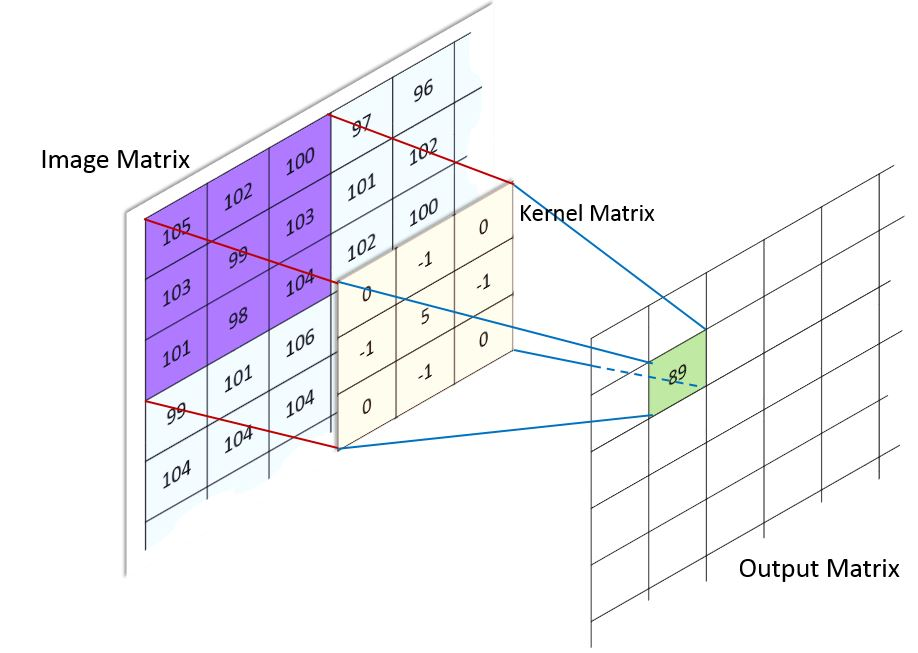
\includegraphics[scale=0.2]{kernel}
	\end{center}
	\begin{itemize}
		\setlength\itemsep{1em}
		\setbeamertemplate{itemize item}[triangle]
		\setbeamercolor{itemize item}{fg=red}
		\item 
			3x3, 5x5, or 7x7, why only odd numbers?
		\item 
			Edge detection
			\begin{itemize}
				\setbeamertemplate{itemize subitem}[circle]
				\setbeamercolor{itemize subitem}{fg=red}
				\item 
					Similarity with human vision
				\item 
					From simple to complex forms
			\end{itemize}
	\end{itemize}
\end{frame}

\begin{frame}{Pooling layers}
	\begin{itemize}
		\setlength\itemsep{1em}
		\setbeamertemplate{itemize item}[triangle]
		\setbeamercolor{itemize item}{fg=red}
		\item 
			Reducing number of information: best way to avoiding \textbf{overfitting} and decreasing 							computation complexity
	\end{itemize}
	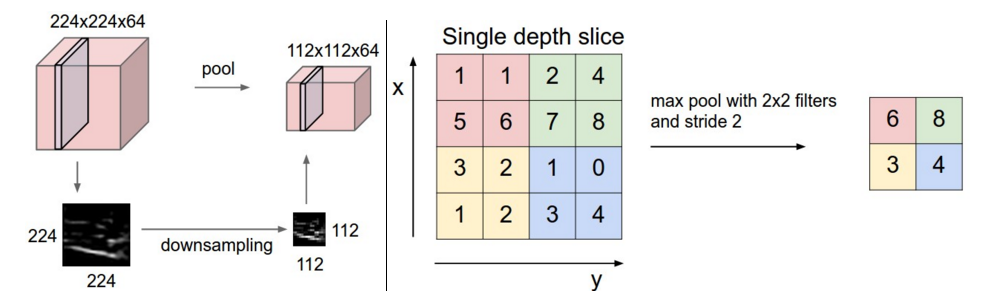
\includegraphics[scale=0.35]{pooling}
\end{frame}

\begin{frame}{Fully connected layers and dropout}
	\begin{itemize}
		\setlength\itemsep{1em}
		\setbeamertemplate{itemize item}[triangle]
		\setbeamercolor{itemize item}{fg=red}
		\item 
			Fully connected layers are the last layer of the CNN
		\item 
			Once the high-level features are recognized, they deal with classifications
	\end{itemize}
	\begin{center}
		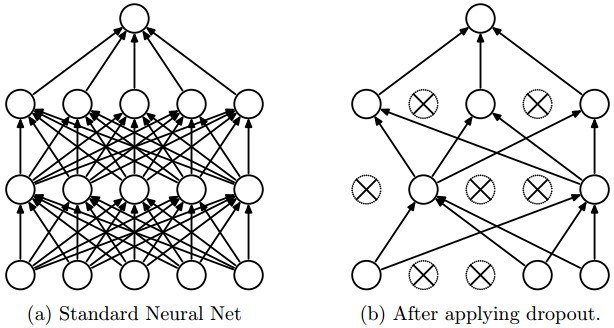
\includegraphics[scale=0.35]{dropout}
	\end{center}
\end{frame}

\begin{frame}{Activation functions}
	\begin{itemize}
		\setlength\itemsep{1em}
		\setbeamertemplate{itemize item}[triangle]
		\setbeamercolor{itemize item}{fg=red}
		\item 
			ReLU
	\end{itemize}
	\begin{center}
		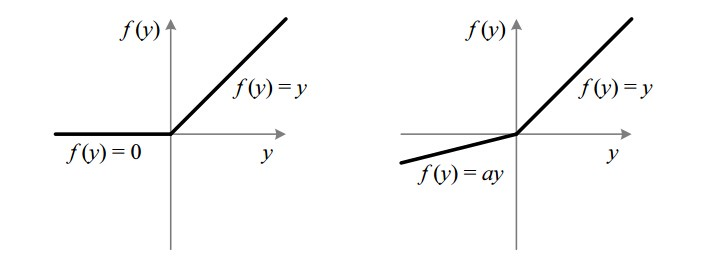
\includegraphics[scale=0.2]{ReLU}
	\end{center}
	\begin{itemize}
		\setlength\itemsep{1em}
		\setbeamertemplate{itemize item}[triangle]
		\setbeamercolor{itemize item}{fg=red}
		\item 
			Softmax
	\end{itemize}
	\begin{center}
		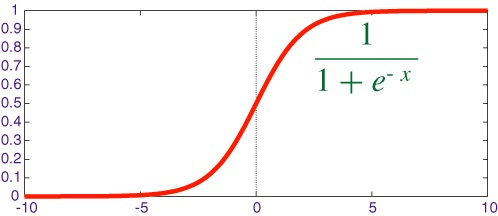
\includegraphics[scale=0.2]{softmax1}
	\end{center}
\end{frame}

\subsection{Dataset}

\begin{frame}{Dataset}
	\begin{itemize}
		\setlength\itemsep{1em}
		\setbeamertemplate{itemize item}[triangle]
		\setbeamercolor{itemize item}{fg=red}
		\item 
			The perfect dataset should be:
			\begin{itemize}
				\setbeamertemplate{itemize subitem}[circle]
				\setbeamercolor{itemize subitem}{fg=red}
				\item 
					made with hundreds of images
				\item 
					different images with different colors to help the network classify them better
			\end{itemize}
		\item 
			How the script works?
			\begin{itemize}
				\setbeamertemplate{itemize subitem}[circle]
				\setbeamercolor{itemize subitem}{fg=red}
				\item 
					It use some OpenCv functions to get hundreds of photos in less than 30 seconds
				\item 
					After that, crop them and saves them
				\item
					This is made to avoid the recognition of unwanted features as background color without 							the need of hundreds of images taken in different places
			\end{itemize}
	\end{itemize}
\end{frame}

\subsection{ImageNet}

\begin{frame}{ImageNet Challenge}
	\begin{itemize}
		\setlength\itemsep{1em}
		\setbeamertemplate{itemize item}[triangle]
		\setbeamercolor{itemize item}{fg=red}
		\item 
			The ImageNet project:
			\begin{itemize}
				\setbeamertemplate{itemize subitem}[circle]
				\setbeamercolor{itemize subitem}{fg=red}
				\item 
					it's a large visual database designed for use in visual object recognition software research
				\item 
					ImageNet contains over 20 thousand categories; a typical category, such as "balloon" or 							"strawberry", contains several hundred images.
				\item
					all the images are labelled and this i fundamental for machine learning works on it
			\end{itemize}
		\item 
			ImageNet Large Scale Visual Recognition Challenge (ILSVRC):
			\begin{itemize}
				\setbeamertemplate{itemize subitem}[circle]
				\setbeamercolor{itemize subitem}{fg=red}
				\item 
					is a competition where research teams evaluate their algorithms on the given data								set(ImageNet)
				\item 
					they compete to achieve higher accuracy on several visual recognition tasks
			\end{itemize}
	\end{itemize}
\end{frame}

\subsection{Inception V3 by Google}

\begin{frame}{Inception network}
	\begin{itemize}
		\setlength\itemsep{1em}
		\setbeamertemplate{itemize item}[triangle]
		\setbeamercolor{itemize item}{fg=red}
		\item 
			Inception networks analize images with different kernel size (in the same conv layer)
	\end{itemize}
	\begin{center}
		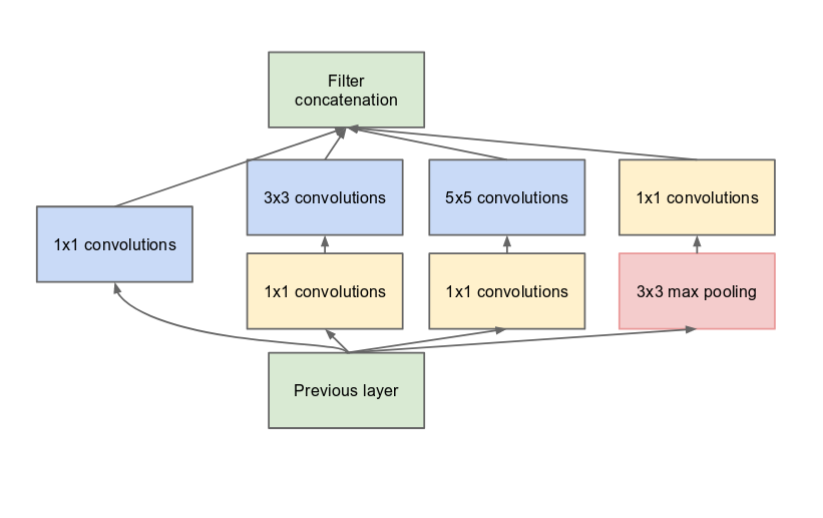
\includegraphics[scale=0.28]{inception}
	\end{center}
	\begin{itemize}
		\setlength\itemsep{1em}
		\setbeamertemplate{itemize item}[triangle]
		\setbeamercolor{itemize item}{fg=red}
		\item 
			Here an example: \href{https://bit.ly/2vBgoO3}{\color{red}GoogleNet}
	\end{itemize}
\end{frame}

\subsection{Tensorflow and retraining}

\begin{frame}{Tensorflow and retraining}
	\begin{itemize}
		\setlength\itemsep{1em}
		\setbeamertemplate{itemize item}[triangle]
		\setbeamercolor{itemize item}{fg=red}
		\item 
			Concept of retraining
		\item 
			Tensorflow-hub: the key to create your own classifier with good result and without a Tesla k80
		\item 
			Everything you need to know about retrain: \href{https://www.tensorflow.org/hub/tutorials/						image_retraining}{\color{red}tensorflow retraining}
	\end{itemize}
\end{frame}

\section{Summary}

\subsection{Conclusion}
\begin{frame}{Conclusion}
	\begin{itemize}
	\setlength\itemsep{1em}
	\setbeamertemplate{itemize item}[triangle]
	\setbeamercolor{itemize item}{fg=red}
	\item 
		Create your own machine learning program using another pre-trained model can help you to build 					something useful without the need of a workstation or cloud computing
	\item 
		This project is only a small example of the potentiality of Tensorflow and the machine learning approach
	\end{itemize}
\end{frame}

\subsection{Future implementation}

\begin{frame}{Future implementation}
	\begin{itemize}
		\setlength\itemsep{1em}
		\setbeamertemplate{itemize item}[triangle]
		\setbeamercolor{itemize item}{fg=red}
		\item 
			Let the users to choose beetwen more pre-trained models
		\item 
			Find the best way to recognize an unknown person (someone who does not have photos yet)
	\end{itemize}
\end{frame}

\subsection{Best bugs}

\begin{frame}{Best bugs}
	\begin{itemize}
		\setlength\itemsep{1em}
		\setbeamertemplate{itemize item}[triangle]
		\setbeamercolor{itemize item}{fg=red}
		\item 
			OpenCv imshow freezing bug on unix like system
		\item 
			Tensorflow-hub requires a tensorflow version that could not work with lots of 									processors(precompiled with AVX activation)
			(\href{https://github.com/tensorflow/tensorflow/issues/17411}{\color{red}Link to issue})
	\end{itemize}
\end{frame}

\appendix
\section<presentation>*{\appendixname}
\subsection<presentation>*{Useful links}

\begin{frame}{Useful links}
	\begin{itemize}
		\setlength\itemsep{1em}
		\setbeamertemplate{itemize item}[triangle]
		\setbeamercolor{itemize item}{fg=red}
		\item 
			Project repository: \href{https://github.com/SimoneCaldarella/faceRecognition}{\color{red}Link to repo}
		\item 
			Tensorflow: \href{https://www.tensorflow.org}{\color{red}Link to Tensorflow page}
		\item 
			OpenCv: \href{https://opencv.org}{\color{red}Link to OpenCv project}
	\end{itemize}
\end{frame}

\end{document}


